%Matteo Kumar - Leonhard Schatt
% Fortgeschrittenes Physikalisches Praktikum

% Teilauswertung Bleach

\section{Bestimmung der Förstereffizienz über Bleichung der Akzeptoren}

Ein alternativer Ansatz zur Bestimmung der Förstereffizienz $E$ ist, die Donorfluoreszenz vor und nach dem Bleichen der Akzeptoren zu betrachten. Denn wird ein 
Teil der Akzeptoren zerstört, so gibt es für einen Donor im angeregten Zustand nur noch einen möglichen Weg, diesen zu verlassen: Das angeregte Elektron relaxiert in den 
Grundzustand unter Aussendung eines Photons; es ist also eine Erhöhung der Donorfluoreszenz zu erwarten und zwar um den Betrag, um den die Sensitized Emission zurückgeht. \\
Um eine Zelle aus der Probe mit CFP und YFP wird eine ROI1 ausgewählt, die gebleicht werden soll. 
Zudem wird in dieser, wie auch in der Membranregion (ROI2) und in einer kleinen Region dieser (ROI3) die Intensität kurz vor bis kurz nach dem Bleichvorgang gemessen. 
In Abb. \ref{bild:bleachROI} ist so eine Zelle dargestellt. Dabei ist die ROI1 in Grün, ROI2 in Violett und ROI3 in Orange dargestellt. In Abb. \ref{bild:bleachPlotD} 
und Abb. \ref{bild:bleachPlotS} sind die Intensitätsverläufe dieser Zelle für den Donor- bzw. SE-Kanal in den selben Farben dargestellt. 
Dabei ist vor allem in den ROIs 2 ud 3, also in denjenigen, in denen die Dichte an Fluorophoren besonders groß ist, zu erkennen, dass zum 
Einen die Donorfluoreszenz nach dem Bleichen einen höheren Wert erreicht. Zum Anderen fällt dort die Intensität im SE-Kanal nach dem 
Bleichvorgang ab.


\begin{figure}[h]
    \centering
    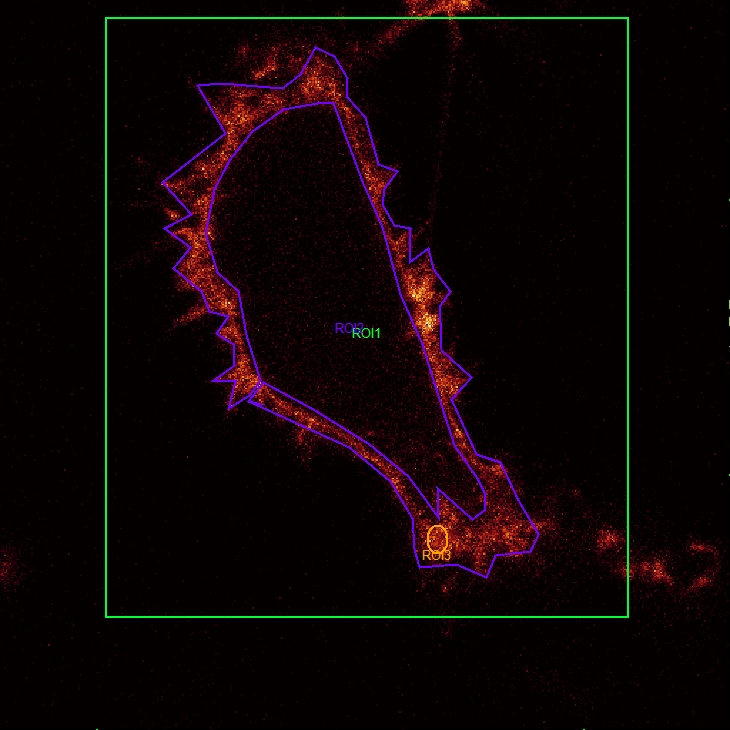
\includegraphics[scale = 0.45]{Bilder/bleachROI.jpg}
    \caption{Bild einer gebleichten Zelle mit CFP und YFP. Dabei sind die ROIs, in denen die Intensitäten gemessen wurden eingezeichnet.}
    \label{bild:bleachROI}
\end{figure}

\begin{figure}[h]
    \centering
    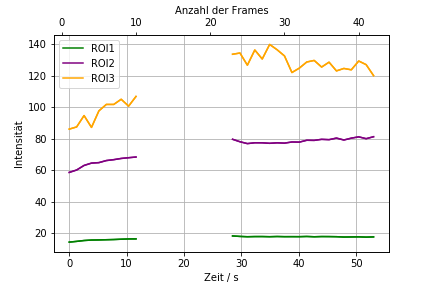
\includegraphics[scale = 0.45]{Bilder/bleachPlotD.png}
    \caption{Verlauf der Intensitäten einer Zelle für verschiedenen ROIs im Donor-Kanal vor, während und nach dem Bleichen.}
    \label{bild:bleachPlotD}
\end{figure}

\begin{figure}[h]
    \centering
    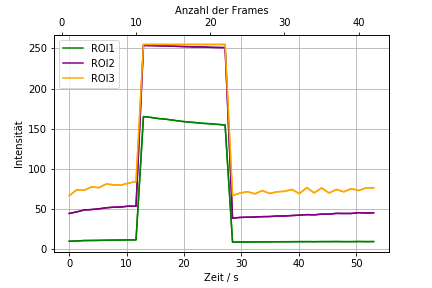
\includegraphics[scale = 0.45]{Bilder/bleachPlotS.png}
    \caption{Verlauf der Intensitäten einer Zelle für verschiedenen ROIs im SE-Kanal vor, während und nach dem Bleichen.}
    \label{bild:bleachPlotS}
\end{figure}